% Options for packages loaded elsewhere
% Options for packages loaded elsewhere
\PassOptionsToPackage{unicode}{hyperref}
\PassOptionsToPackage{hyphens}{url}
\PassOptionsToPackage{dvipsnames,svgnames,x11names}{xcolor}
%
\documentclass[
  french,
]{report}
\usepackage{xcolor}
\usepackage{amsmath,amssymb}
\setcounter{secnumdepth}{-\maxdimen} % remove section numbering
\usepackage{iftex}
\ifPDFTeX
  \usepackage[T1]{fontenc}
  \usepackage[utf8]{inputenc}
  \usepackage{textcomp} % provide euro and other symbols
\else % if luatex or xetex
  \usepackage{unicode-math} % this also loads fontspec
  \defaultfontfeatures{Scale=MatchLowercase}
  \defaultfontfeatures[\rmfamily]{Ligatures=TeX,Scale=1}
\fi
\usepackage{lmodern}
\ifPDFTeX\else
  % xetex/luatex font selection
\fi
% Use upquote if available, for straight quotes in verbatim environments
\IfFileExists{upquote.sty}{\usepackage{upquote}}{}
\IfFileExists{microtype.sty}{% use microtype if available
  \usepackage[]{microtype}
  \UseMicrotypeSet[protrusion]{basicmath} % disable protrusion for tt fonts
}{}
\makeatletter
\@ifundefined{KOMAClassName}{% if non-KOMA class
  \IfFileExists{parskip.sty}{%
    \usepackage{parskip}
  }{% else
    \setlength{\parindent}{0pt}
    \setlength{\parskip}{6pt plus 2pt minus 1pt}}
}{% if KOMA class
  \KOMAoptions{parskip=half}}
\makeatother
% Make \paragraph and \subparagraph free-standing
\makeatletter
\ifx\paragraph\undefined\else
  \let\oldparagraph\paragraph
  \renewcommand{\paragraph}{
    \@ifstar
      \xxxParagraphStar
      \xxxParagraphNoStar
  }
  \newcommand{\xxxParagraphStar}[1]{\oldparagraph*{#1}\mbox{}}
  \newcommand{\xxxParagraphNoStar}[1]{\oldparagraph{#1}\mbox{}}
\fi
\ifx\subparagraph\undefined\else
  \let\oldsubparagraph\subparagraph
  \renewcommand{\subparagraph}{
    \@ifstar
      \xxxSubParagraphStar
      \xxxSubParagraphNoStar
  }
  \newcommand{\xxxSubParagraphStar}[1]{\oldsubparagraph*{#1}\mbox{}}
  \newcommand{\xxxSubParagraphNoStar}[1]{\oldsubparagraph{#1}\mbox{}}
\fi
\makeatother


\usepackage{longtable,booktabs,array}
\usepackage{calc} % for calculating minipage widths
% Correct order of tables after \paragraph or \subparagraph
\usepackage{etoolbox}
\makeatletter
\patchcmd\longtable{\par}{\if@noskipsec\mbox{}\fi\par}{}{}
\makeatother
% Allow footnotes in longtable head/foot
\IfFileExists{footnotehyper.sty}{\usepackage{footnotehyper}}{\usepackage{footnote}}
\makesavenoteenv{longtable}
\usepackage{graphicx}
\makeatletter
\newsavebox\pandoc@box
\newcommand*\pandocbounded[1]{% scales image to fit in text height/width
  \sbox\pandoc@box{#1}%
  \Gscale@div\@tempa{\textheight}{\dimexpr\ht\pandoc@box+\dp\pandoc@box\relax}%
  \Gscale@div\@tempb{\linewidth}{\wd\pandoc@box}%
  \ifdim\@tempb\p@<\@tempa\p@\let\@tempa\@tempb\fi% select the smaller of both
  \ifdim\@tempa\p@<\p@\scalebox{\@tempa}{\usebox\pandoc@box}%
  \else\usebox{\pandoc@box}%
  \fi%
}
% Set default figure placement to htbp
\def\fps@figure{htbp}
\makeatother



\ifLuaTeX
\usepackage[bidi=basic]{babel}
\else
\usepackage[bidi=default]{babel}
\fi
% get rid of language-specific shorthands (see #6817):
\let\LanguageShortHands\languageshorthands
\def\languageshorthands#1{}


\setlength{\emergencystretch}{3em} % prevent overfull lines

\providecommand{\tightlist}{%
  \setlength{\itemsep}{0pt}\setlength{\parskip}{0pt}}



 


\usepackage{booktabs}
\usepackage{caption}
\usepackage{longtable}
\usepackage{colortbl}
\usepackage{array}
\usepackage{anyfontsize}
\usepackage{multirow}
\usepackage{multirow}
\usepackage{longtable}
\makeatletter
\@ifpackageloaded{caption}{}{\usepackage{caption}}
\AtBeginDocument{%
\ifdefined\contentsname
  \renewcommand*\contentsname{Table des matières}
\else
  \newcommand\contentsname{Table des matières}
\fi
\ifdefined\listfigurename
  \renewcommand*\listfigurename{Liste des Figures}
\else
  \newcommand\listfigurename{Liste des Figures}
\fi
\ifdefined\listtablename
  \renewcommand*\listtablename{Liste des Tables}
\else
  \newcommand\listtablename{Liste des Tables}
\fi
\ifdefined\figurename
  \renewcommand*\figurename{Figure}
\else
  \newcommand\figurename{Figure}
\fi
\ifdefined\tablename
  \renewcommand*\tablename{Table}
\else
  \newcommand\tablename{Table}
\fi
}
\@ifpackageloaded{float}{}{\usepackage{float}}
\floatstyle{ruled}
\@ifundefined{c@chapter}{\newfloat{codelisting}{h}{lop}}{\newfloat{codelisting}{h}{lop}[chapter]}
\floatname{codelisting}{Listing}
\newcommand*\listoflistings{\listof{codelisting}{Liste des Listings}}
\makeatother
\makeatletter
\makeatother
\makeatletter
\@ifpackageloaded{caption}{}{\usepackage{caption}}
\@ifpackageloaded{subcaption}{}{\usepackage{subcaption}}
\makeatother
\usepackage{bookmark}
\IfFileExists{xurl.sty}{\usepackage{xurl}}{} % add URL line breaks if available
\urlstyle{same}
\hypersetup{
  pdftitle={Test Ch01 --- Description},
  pdflang={fr},
  colorlinks=true,
  linkcolor={blue},
  filecolor={Maroon},
  citecolor={Blue},
  urlcolor={Blue},
  pdfcreator={LaTeX via pandoc}}


\title{Test Ch01 --- Description}
\author{}
\date{}
\begin{document}
\maketitle


\chapter{Map test --- tmap static}\label{map-test-tmap-static}

\begin{figure}[H]

{\centering \pandocbounded{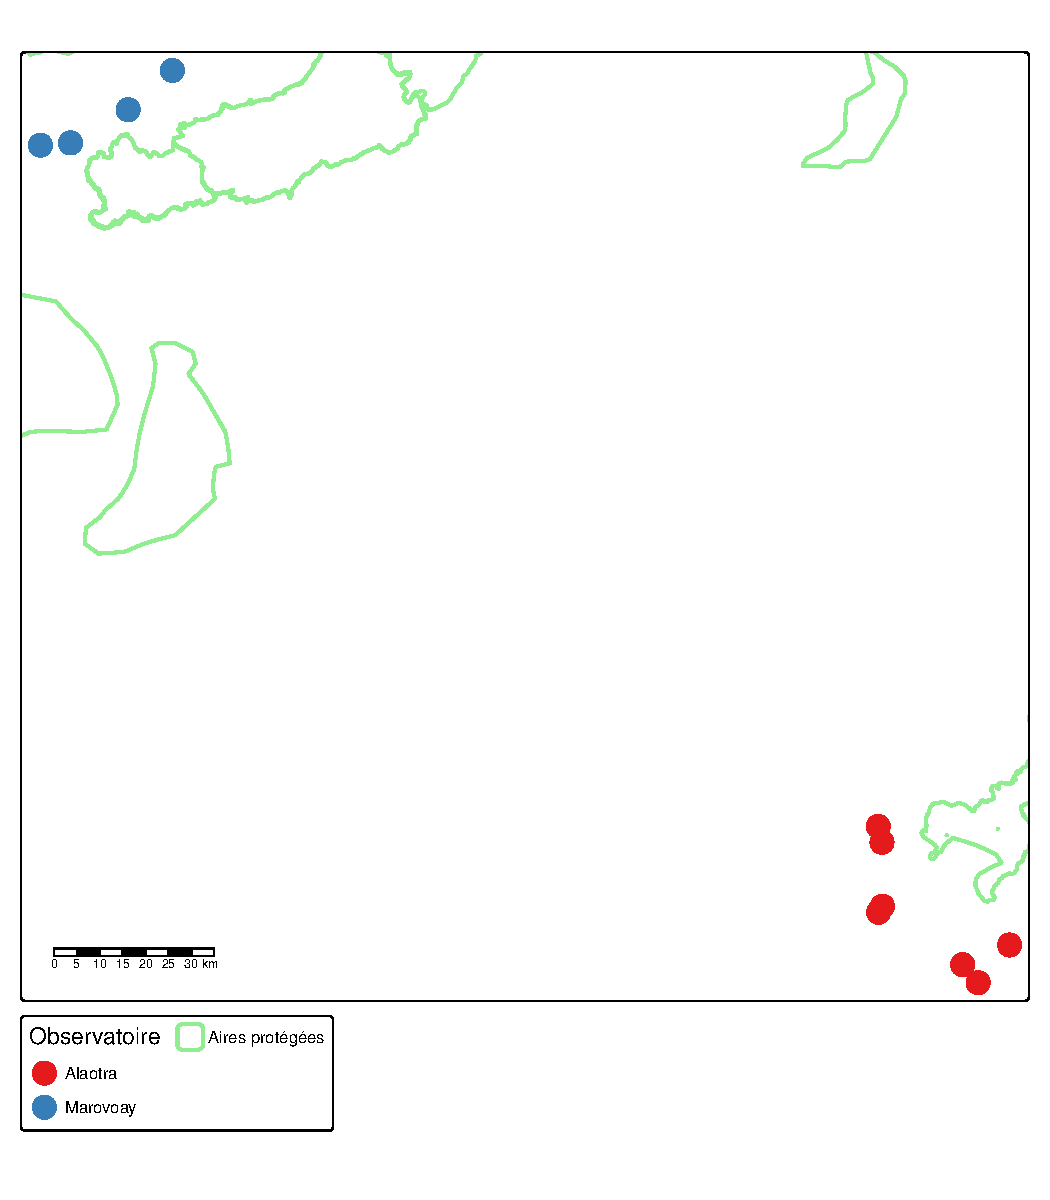
\includegraphics[keepaspectratio]{test_ch01_files/figure-pdf/carte_sites-1.pdf}}

}

\caption{Localisation approximative des fokontany enquêtés}

\end{figure}%

\chapter{Tables from Ch01}\label{tables-from-ch01}

\section{Table: Répartition des
ménages}\label{table-ruxe9partition-des-muxe9nages}

\begin{table}

\caption{\label{tbl-men-obs}Répartition des ménages et des individus
selon les observatoires}

\centering{

\fontsize{12.0pt}{14.0pt}\selectfont
\begin{tabular*}{\linewidth}{@{\extracolsep{\fill}}lrrrr}
\toprule
Observatoire & M\\'enages & Individus & \% m\\'enages & \% individus \\ 
\midrule\addlinespace[2.5pt]
Marovoay & 519 & 2 297 & 50.6 & 53.8 \\ 
Alaotra & 507 & 1 975 & 49.4 & 46.2 \\ 
{\bfseries \cellcolor[HTML]{B0E0E6}{Ensemble}} & {\bfseries \cellcolor[HTML]{B0E0E6}{1 026}} & {\bfseries \cellcolor[HTML]{B0E0E6}{4 272}} & {\bfseries \cellcolor[HTML]{B0E0E6}{100.0}} & {\bfseries \cellcolor[HTML]{B0E0E6}{100.0}} \\ 
\bottomrule
\end{tabular*}
\begin{minipage}{\linewidth}
\textbf{Source : Enquête auprès des OR 2025}\\
\end{minipage}

}

\end{table}%

\section{Table: Dénombrement}\label{table-duxe9nombrement}

\begin{table}

\caption{\label{tbl-denombrement}Dénombrement et taux de sondage par
observatoire}

\centering{

\fontsize{12.0pt}{14.0pt}\selectfont
\begin{tabular*}{\linewidth}{@{\extracolsep{\fill}}lrrrr}
\toprule
Observatoire & Toits d\\'enombr\\'es & M\\'enages d\\'enombr\\'es & M\\'enages enqu\^et\\'es & Taux de sondage (\%) \\ 
\midrule\addlinespace[2.5pt]
Alaotra & 6 142 & 6 210 & 507 & 8.2 \\ 
Marovoay & 2 370 & 2 506 & 519 & 20.7 \\ 
\bottomrule
\end{tabular*}
\begin{minipage}{\linewidth}
\textbf{Source : Synthèse Dénombrement OR 2025 \& Enquête auprès des OR 2025}\\
\end{minipage}

}

\end{table}%

\section{Table: Ménages par hameau
(grouped)}\label{table-muxe9nages-par-hameau-grouped}

\begin{table}

\caption{\label{tbl-men-hameau}Répartition des ménages enquêtés par
hameau}

\centering{

\fontsize{12.0pt}{14.0pt}\selectfont
\begin{tabular*}{\linewidth}{@{\extracolsep{\fill}}lrr}
\toprule
Hameau & M\\'enages & \% obs. \\ 
\midrule\addlinespace[2.5pt]
\multicolumn{3}{l}{{\bfseries \cellcolor[HTML]{B0E0E6}{Alaotra}}} \\[2.5pt] 
\midrule\addlinespace[2.5pt]
Avaradrano & 90 & 17.8 \\ 
Feramanga Atsimo & 89 & 17.6 \\ 
Mangabe & 73 & 14.4 \\ 
Ambatomanga & 68 & 13.4 \\ 
Ambodivoara & 58 & 11.4 \\ 
Ambohidrony & 52 & 10.3 \\ 
Analamiranga & 46 & 9.1 \\ 
Ambatoharanana & 31 & 6.1 \\ 
{\bfseries \cellcolor[HTML]{CECECE}{Ensemble}} & {\bfseries \cellcolor[HTML]{CECECE}{507}} & {\bfseries \cellcolor[HTML]{CECECE}{100.0}} \\ 
\midrule\addlinespace[2.5pt]
\multicolumn{3}{l}{{\bfseries \cellcolor[HTML]{B0E0E6}{Marovoay}}} \\[2.5pt] 
\midrule\addlinespace[2.5pt]
Ampijoroa & 143 & 27.6 \\ 
Madiromiongana & 137 & 26.4 \\ 
Bepako & 123 & 23.7 \\ 
Maroala & 116 & 22.4 \\ 
{\bfseries \cellcolor[HTML]{CECECE}{Ensemble}} & {\bfseries \cellcolor[HTML]{CECECE}{519}} & {\bfseries \cellcolor[HTML]{CECECE}{100.0}} \\ 
\bottomrule
\end{tabular*}
\begin{minipage}{\linewidth}
\textbf{Source : Enquête auprès des OR 2025}\\
\end{minipage}

}

\end{table}%

\section{Figure: Chronogramme}\label{figure-chronogramme}

\begin{figure}

\centering{

\pandocbounded{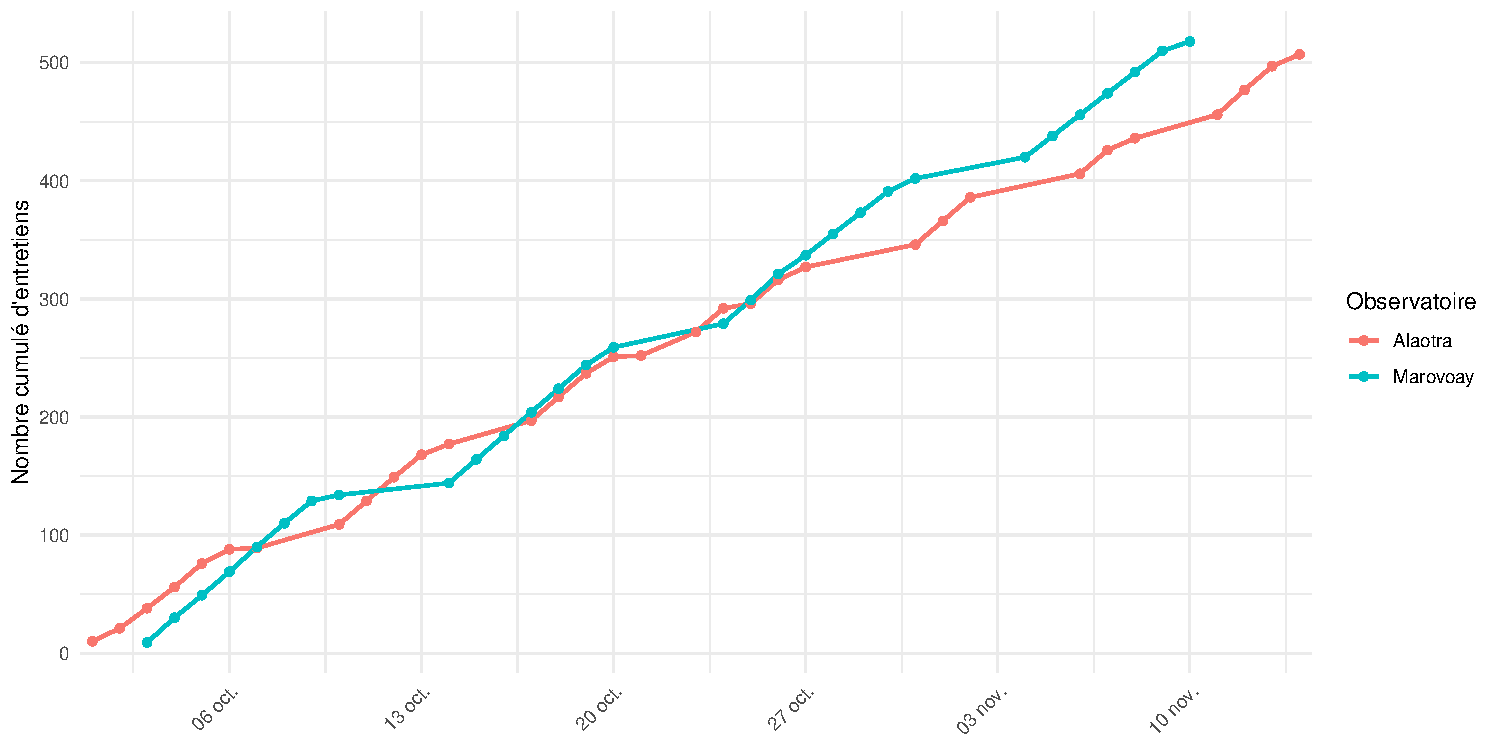
\includegraphics[keepaspectratio]{test_ch01_files/figure-pdf/fig-chronogramme-1.pdf}}

}

\caption{\label{fig-chronogramme}Fréquences cumulées des entretiens par
observatoire}

\end{figure}%

\section{Figure: Enquêteurs}\label{figure-enquuxeateurs}

\begin{figure}

\centering{

\pandocbounded{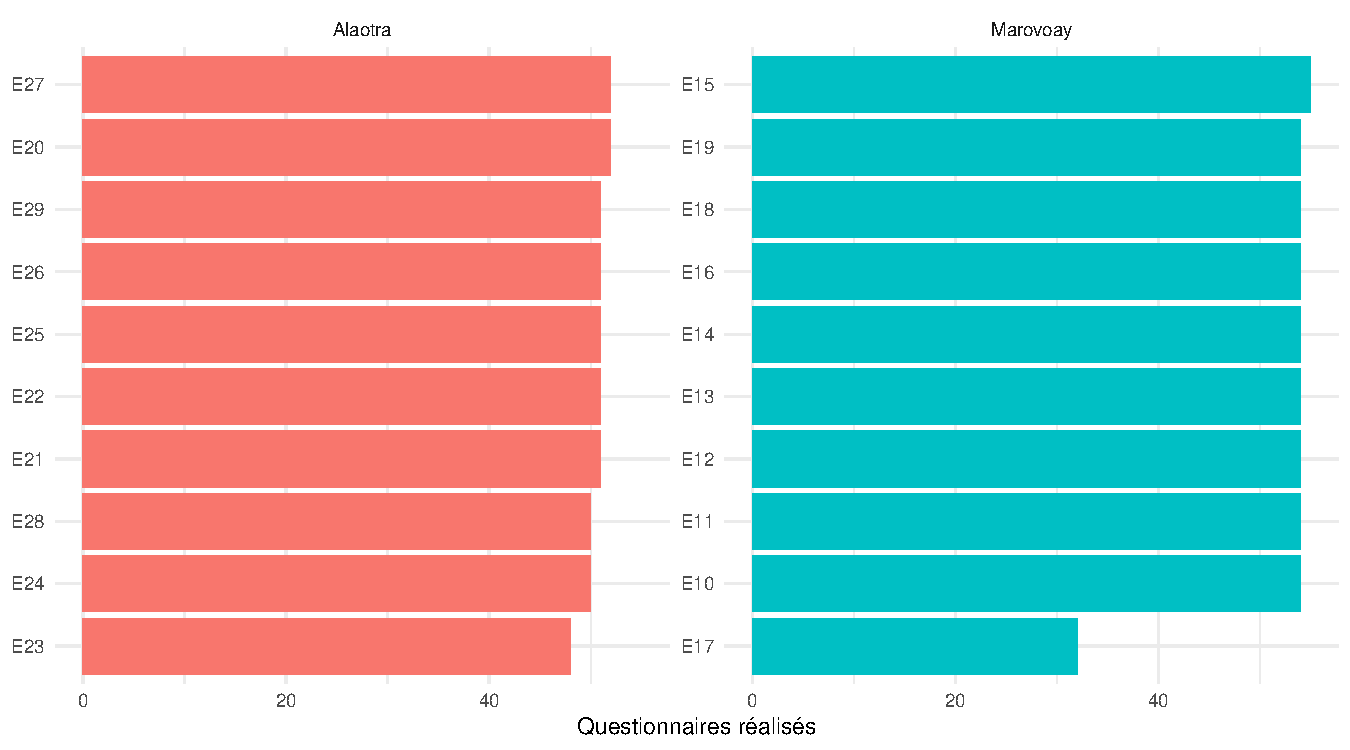
\includegraphics[keepaspectratio]{test_ch01_files/figure-pdf/fig-enqueteurs-1.pdf}}

}

\caption{\label{fig-enqueteurs}Nombre de questionnaires par enquêteur et
observatoire}

\end{figure}%

\section{Table: Superviseurs (wide)}\label{table-superviseurs-wide}

\begin{table}

\caption{\label{tbl-superviseurs}Nombre de questionnaires supervisés par
superviseur}

\centering{

\fontsize{12.0pt}{14.0pt}\selectfont
\begin{tabular*}{\linewidth}{@{\extracolsep{\fill}}lrr}
\toprule
{\bfseries \cellcolor[HTML]{DCDCDC}{Superviseur}} & {\bfseries \cellcolor[HTML]{DCDCDC}{Alaotra}} & {\bfseries \cellcolor[HTML]{DCDCDC}{Marovoay}} \\ 
\midrule\addlinespace[2.5pt]
S01 & 172 & 86 \\ 
S02 & 166 & 217 \\ 
S03 & 169 & 216 \\ 
\bottomrule
\end{tabular*}
\begin{minipage}{\linewidth}
\textbf{Source : Enquête auprès des OR 2025}\\
\end{minipage}

}

\end{table}%




\end{document}
